\documentclass{article}
\usepackage[utf8]{inputenc}
\usepackage[italian]{babel}
\usepackage{amsmath}
\usepackage{amssymb}
\usepackage{siunitx}
\usepackage{tabularray}
\usepackage{graphicx}
\usepackage{float}
\usepackage{minted}
\usepackage[bottom]{footmisc}
\usepackage[page]{appendix}
\newcommand*{\diam}{\varnothing}
\newcommand*{\best}[1]{{#1}_\text{best}}
\newcommand*{\bestp}[1]{{\left(#1\right)}_\text{best}}
\newcommand*{\pbest}[1]{\left({#1}_\text{best}\right)}
\newcommand*{\pbestp}[1]{\left({\left(#1\right)}_\text{best}\right)}
\newcommand*{\errrel}[1]{\frac{\delta #1}{{#1}_\text{best}}}
\title{
    Laboratorio di Fisica 1\\
    R5: Misura del modulo di scorrimento di un filo
}
\author{Gruppo 17: Bergamaschi Riccardo, Graiani Elia, Moglia Simone}
\date{22/11/2023 – 29/11/2023}
\makeindex
\begin{document}

\maketitle

\begin{abstract}
    Il gruppo di lavoro ha misurato la costante torsionale di quattro
    fili metallici, al fine di verificare il modulo di scorrimento dei
    rispettivi materiali.
\end{abstract}

\section{Materiali e strumenti di misura utilizzati}
\begin{center}
    \begin{tblr}{ |Q[l,m]|Q[c,m]|Q[c,m]|Q[c,m]| }
        \hline
        \textbf{Strumento di misura} & \textbf{\:\:\:\:\:Soglia\:\:\:\:\:} & \textbf{Portata} & \textbf{Sensibilità} \\
        \hline
        Sensore di rotazione & $\qty{0.002}{rad}$ & N./A. & $\qty{0.002}{rad}$ \\
        \hline[dashed]
        Cronometro & $\qty{0.001}{s}$ & N./A. & $\qty{0.001}{s}$ \\
        \hline[dashed]
        Metro & $\qty{0.1}{cm}$ & $\qty{300.0}{cm}$ & $\qty{0.1}{cm}$ \\
        \hline[dashed]
        Calibro ventesimale & $\qty{0.05}{mm}$ & $\qty{150.00}{mm}$ & $\qty{0.05}{mm}$ \\
        \hline[dashed]
        Micrometro ad asta filettata & $\qty{0.01}{mm}$ & $\qty{25.00}{mm}$ & $\qty{0.01}{mm}$ \\
        \hline[dashed]
        Bilancia di precisione & $\qty{0.01}{g}$ & $\qty{6200.00}{g}$ & $\qty{0.01}{g}$ \\
        \hline
        \hline
        \textbf{Altro} & \SetCell[c=3]{l} \textbf{Descrizione/Note} \\
        \hline
        {Quattro fili inestensibili} & \SetCell[c=3]{l} {
            Distinguibili per diametro e materiale. \\
            Li indicheremo con $1,2,3,4$.
        } \\
        \hline[dashed]
        {Tre cilindri \\ (con masse e raggi distinti)} & \SetCell[c=3]{l} {
            Indicheremo con $A,B,C$ i tre cilindri e \\
            con $0$, $A+B$, $A+C$,
            $B+C$ e $A+B+C$ \\
            le loro combinazioni.
            % Tutti questi saranno qui chiamati “carichi”.
            } \\
        \hline[dashed]
        {Struttura portante \\ e parti mobili} & \SetCell[c=3]{l} {
            % "IL FILO È IL SOGGETTO DEL PENDOLO"
            Un disco, ruotando, provoca \\
            una deformazione elastica al filo ad esso \\
            fissato lungo l'asse di rotazione.
        } \\
        \hline
    \end{tblr}
\end{center}

\section{Esperienza e procedimento di misura}

\begin{enumerate}
    \item
        Misuriamo le masse dei cilindri con la bilancia di precisione
        e i rispettivi diametri con il calibro ventesimale.
    \item
        Con il metro a nastro e il micrometro ad asta filettata misuriamo,
        rispettivamente, lunghezza e diametro dei fili.
    \item
        Per ogni filo e per ogni combinazione di cilindri:
    \begin{enumerate}
        \item
            Fissiamo il filo al sistema, in modo tale che l'estremità
            inferiore sia vincolata alla struttura, mentre quella superiore
            al disco rotante; posizioniamo poi
            i cilindri sopra al disco, con l'asse centrale allineato
            a quello del disco stesso.
        \item
            Avviamo l'acquisizione dell'angolo in funzione del tempo
            ($\theta(t)$, lo definiremo formalmente più avanti).
        \item
            Ruotando il disco di un angolo prefissato $\theta_0$,
            diamo inizio al moto armonico del pendolo.
            Acquisiamo dati fino all'arresto del moto.
    \end{enumerate}
\end{enumerate}

\section{Analisi dei dati raccolti e conclusioni}
\emph{\textbf{Nota.}
Avendo valutato gli errori sulle grandezze misurate direttamente
come piccoli, casuali e indipendenti, per svolgere ogni calcolo
abbiamo utilizzato la tradizionale propagazione degli errori.
}

\subsection{Costante torsionale e modulo di scorrimento}

Di seguito riportiamo massa, diametro e momento d'inerzia\footnote{
    Il momento d'inerzia è stato calcolato approssimando questi oggetti
    a cilindri di densità uniforme e raggio e altezza costanti, in rotazione
    attorno ad un asse verticale passante per il loro centro:
    \[I_i = \frac{1}{2} m_i \left(\frac{d_i}{2}\right)^2 = \frac{1}{8}m_i d_i^2\]
} dei tre cilindretti:

\begin{center}
\begin{tblr}{ |c|c|c|c| }
    \hline
    $i$ & $m_i\;\;(\unit{g})$ & $d_i\;\;(\unit{cm})$ & $I_i\;\;(10^{-4}\,\unit{kg\,m^2})$ \\
    \hline
    % 0 & 473.02 & 9.845 & \\
    A & $344.07 \pm 0.01$ & $9.045 \pm 0.005$ & $3.519 \pm 0.004$ \\
    B & $429.65 \pm 0.01$ & $5.985 \pm 0.005$ & $1.924 \pm 0.003$ \\
    C & $473.02 \pm 0.01$ & $5.200 \pm 0.005$ & $1.599 \pm 0.003$ \\
    \hline
\end{tblr}
\end{center}

Fissiamo un sistema di riferimento inerziale, solidale all'apparato,
a coordinate cilindriche\footnote{
    Le coordinate di un punto $P$ in questo sistema di riferimento sono
    definite come segue: detta $\vec{r}$ la proiezione di $\overrightarrow{OP}$
    sul piano per $O$ normale a $\hat{z}$,
    $\theta$ è l'angolo piano orientato fra $\hat{x}$ e $\vec{r}$,
    $r$ è la norma di $\vec{r}$ e
    $h$ è la posizione lungo $\hat{z}$ della proiezione di $P$ su
    $\hat{z}$ stesso.
} $(\theta, r, h)$, con versore $\hat{z}$ giacente
lungo l'asse di rotazione del filo (antiparallelo a $\vec{g}$),
origine $O$ e versore $\hat{x}$ contenuti nel piano sul quale vengono appoggiati
i cilindri. Sia inoltre $P$ un punto materiale qualunque solidale all'estremità
superiore del filo (e quindi anche ai cilindretti) che, con il filo a riposo,
si trovi sul piano $xOz$.
Allora, \emph{trascurando gli attriti}, il moto di $P$ è caratterizzato da:
\[\theta(t) = \theta_0 \cos(\omega t)\]
La pulsazione $\omega$ di questo moto armonico dipende dal momento d'inerzia
complessivo $I_\text{tot}$ dei corpi solidali all'estremità mobile del filo,
nonché dalle caratteristiche del filo stesso. Queste ultime vengono riassunte
nella \emph{costante torsionale} $C$. In particolare:
\[ C = I_\text{tot}\,\omega^2 \]
Detto $T = 2\pi / \omega$ il periodo del moto armonico, si ottiene:
\[ I_\text{tot} = \frac{C}{4\pi^2}\,T^2 \]
Detto $I_0$ il momento d'inerzia che rimane costante\footnote{
    $I_0$ include, ad esempio, il momento d'inerzia del disco su cui
    era possibile appoggiare i cilindretti, nonché quello della parte mobile
    del sensore di rotazione.
},
al variare dei cilindretti ($\text{Cil}$) posizionati sopra al filo, si ha:
\[ \sum_{i\,\in\,\text{Cil}}\!\!I_i = \frac{C}{4\pi^2}\,T^2 - I_0 \]
Da questa relazione, tramite una regressione lineare (pesata\footnote{
    Gli errori assoluti su $I$ variano da punto a punto.
}), è possibile
ottenere una stima piuttosto precisa dei valori di $C$ e $I_0$.

\begin{center}
    \begin{figure}[H]
        % trim={< v > ^}
        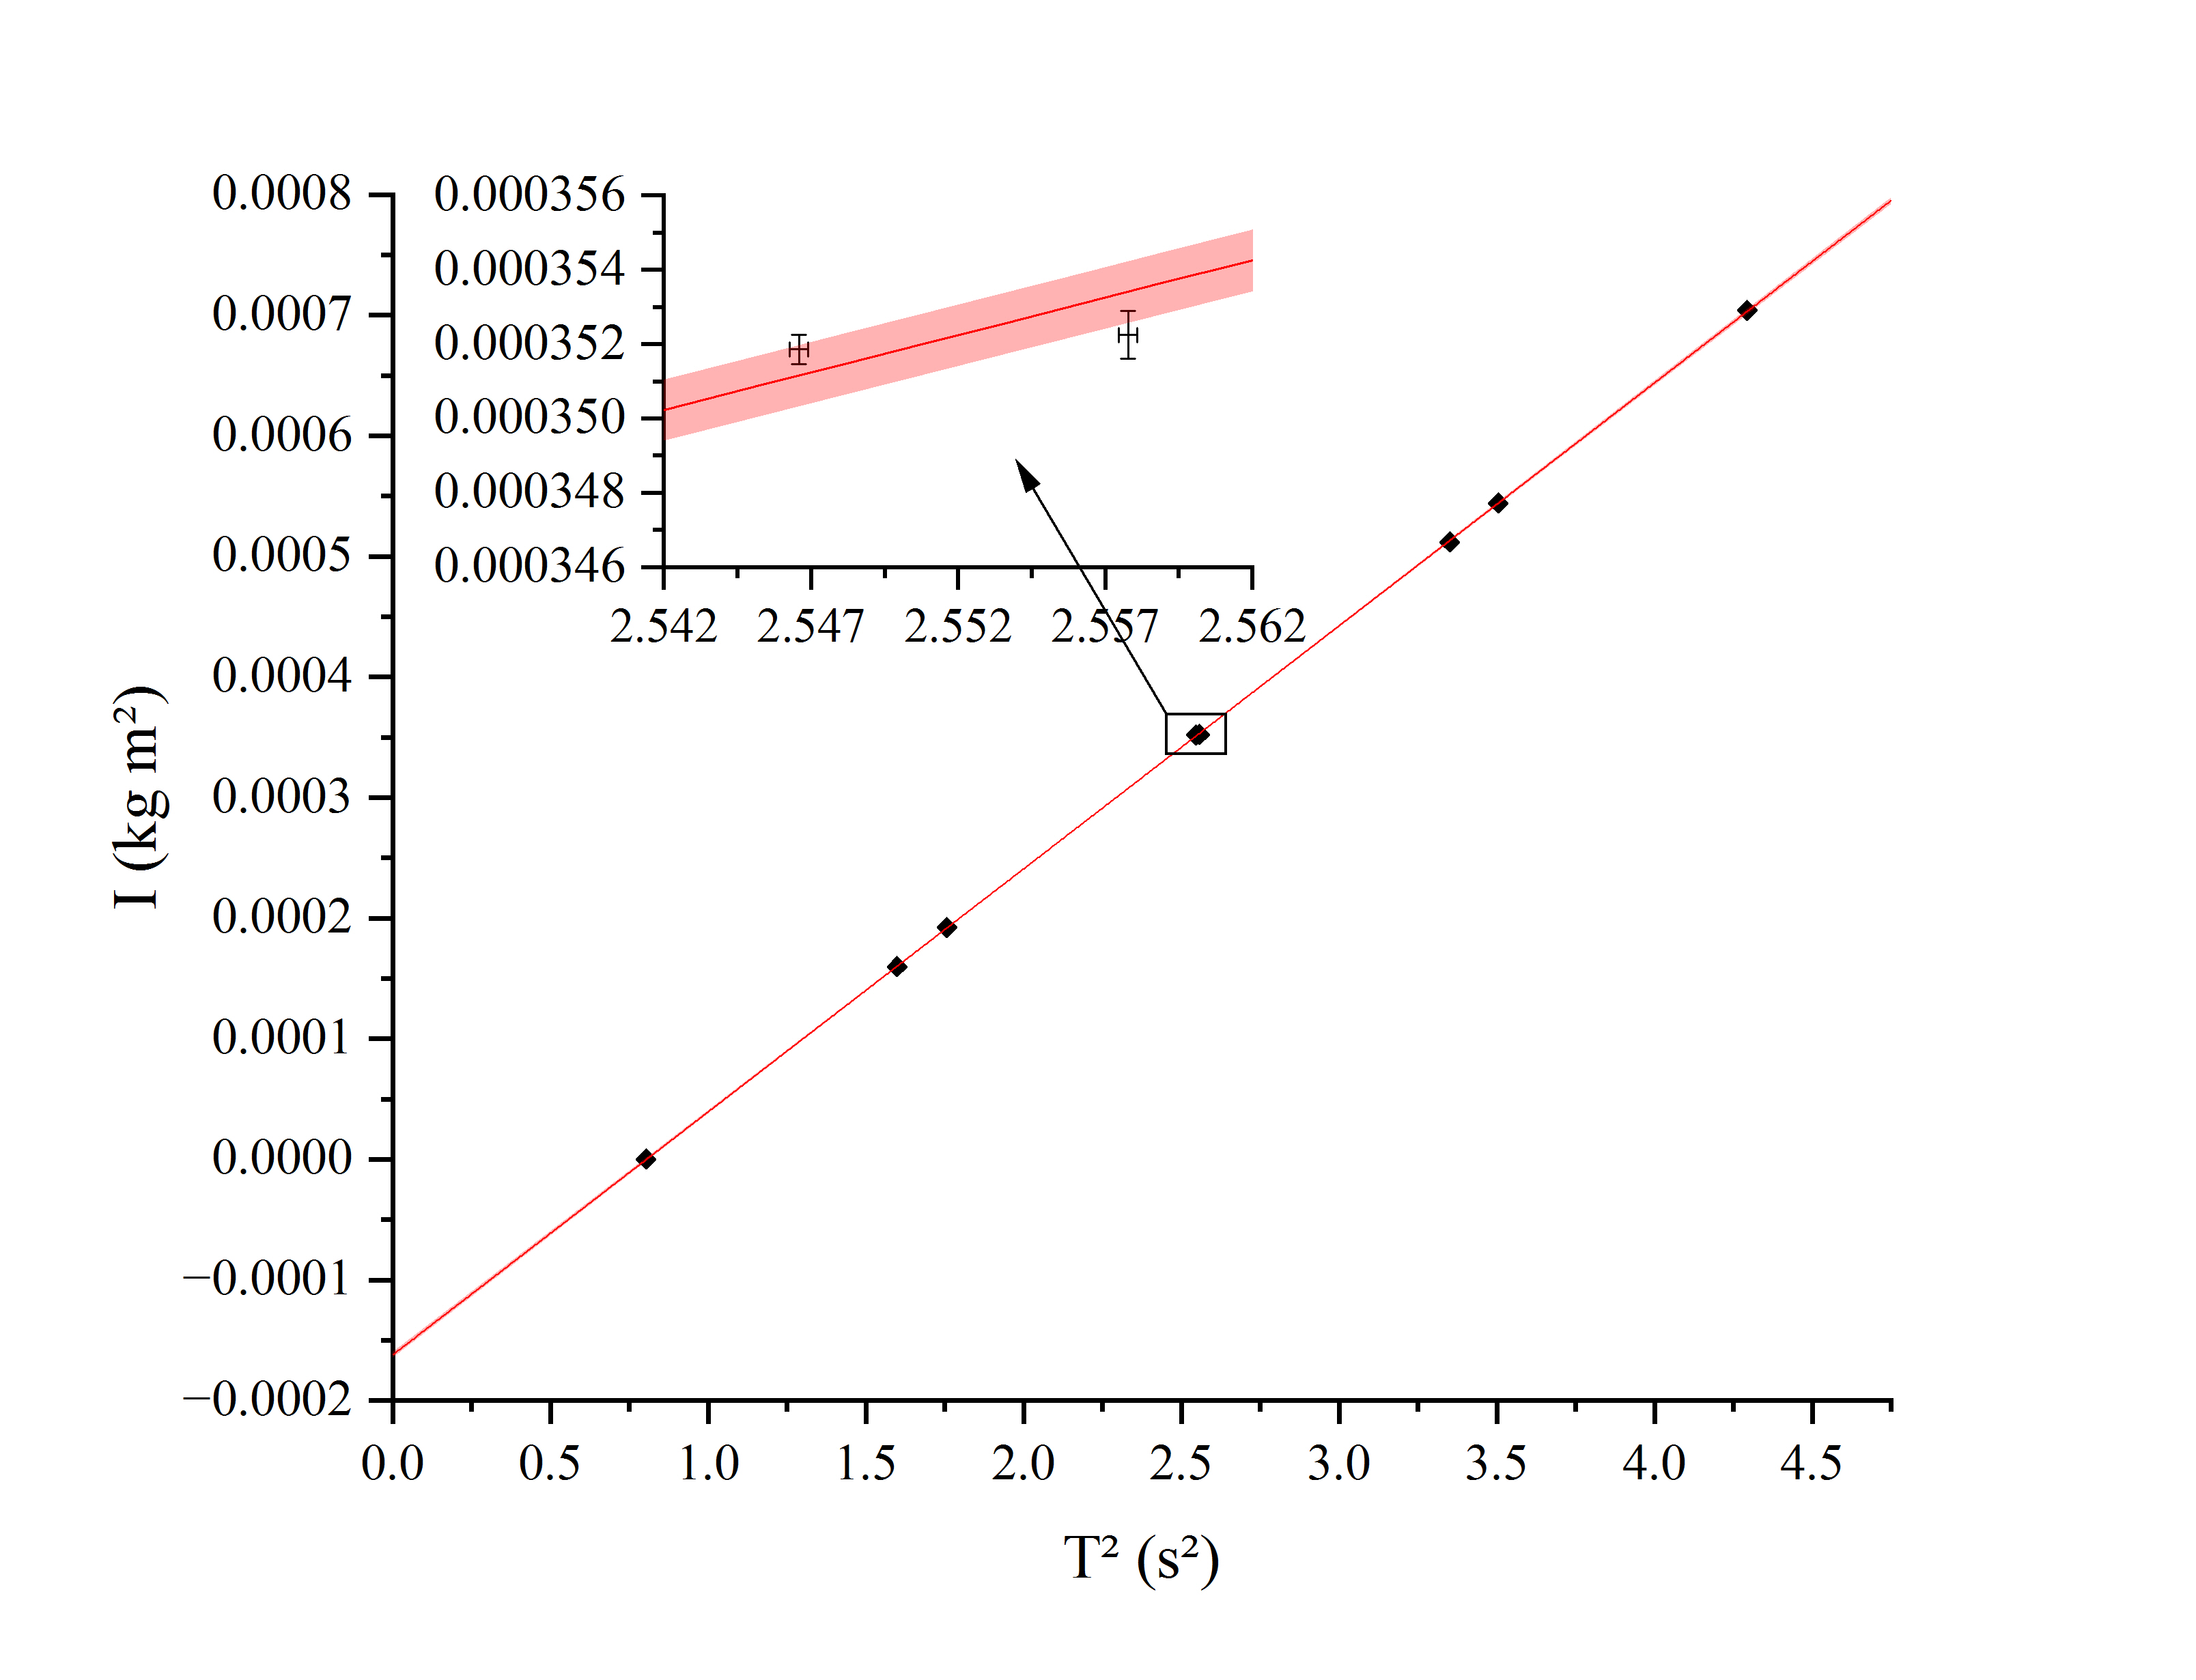
\includegraphics[trim={1.4cm .5cm 3.1cm 2.1cm},clip,width=.5\textwidth]{img/Reg1.jpg}
        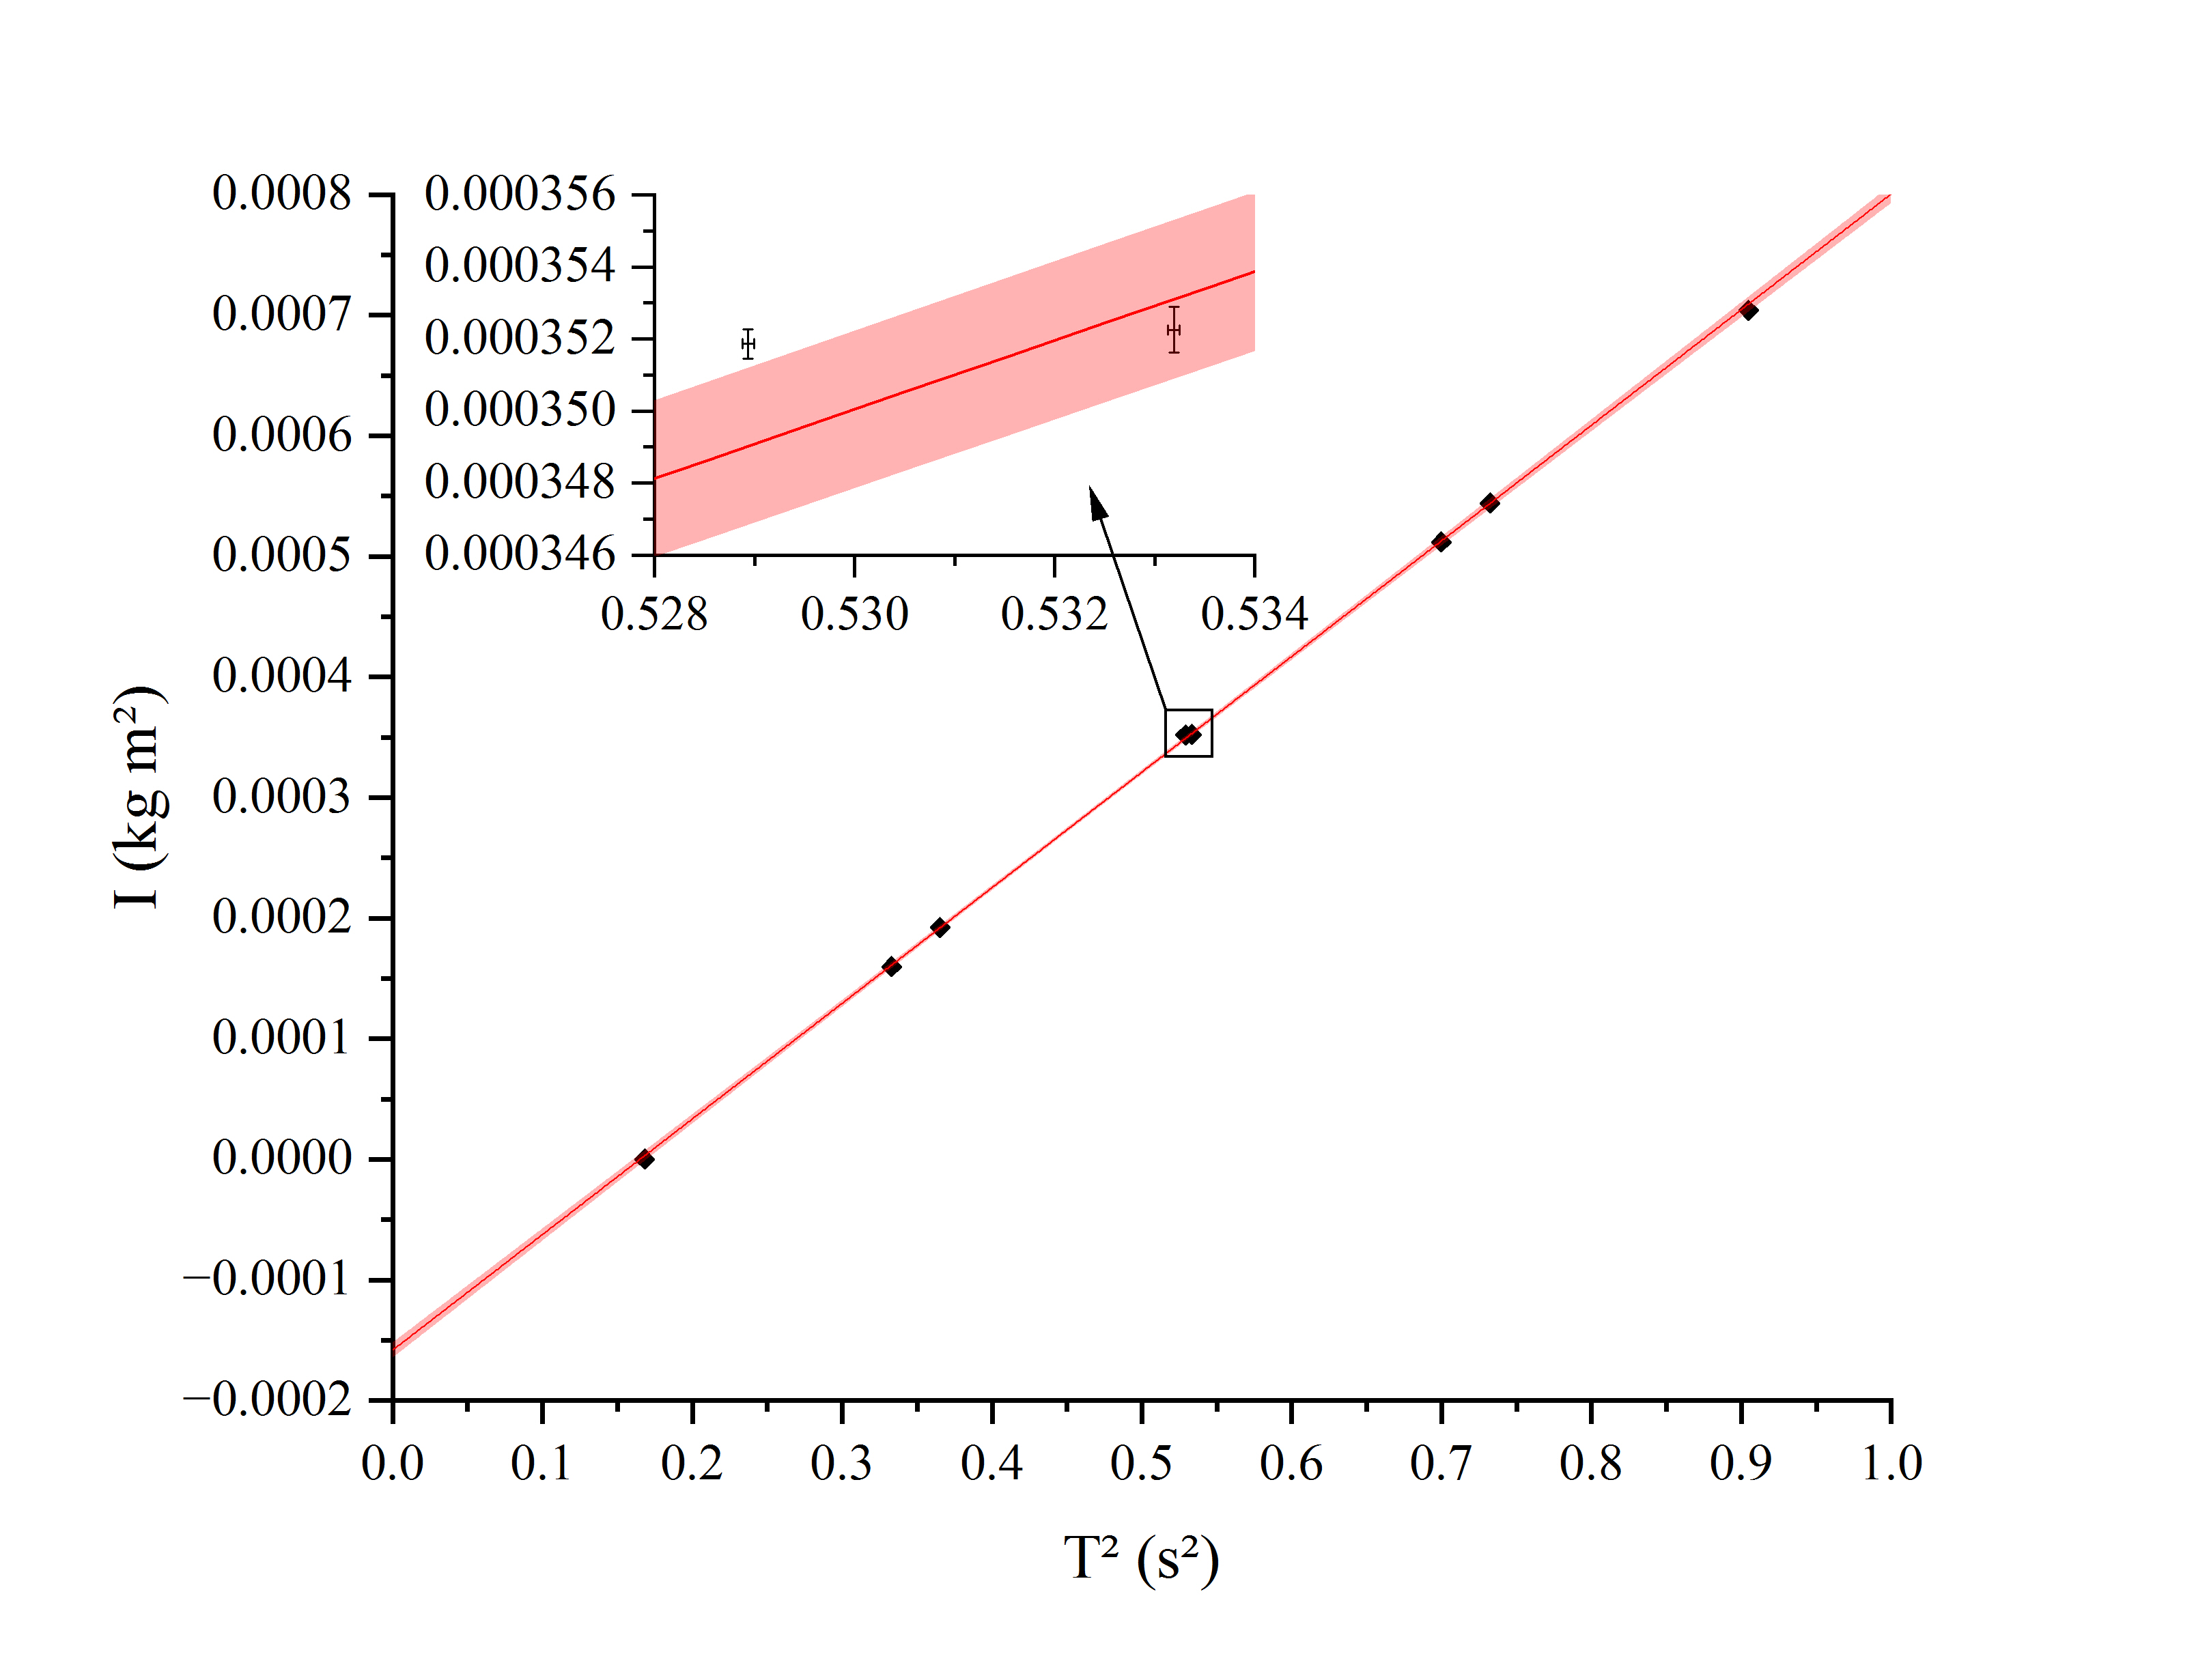
\includegraphics[trim={1.4cm .5cm 3.1cm 2.1cm},clip,width=.5\textwidth]{img/Reg2.jpg}
        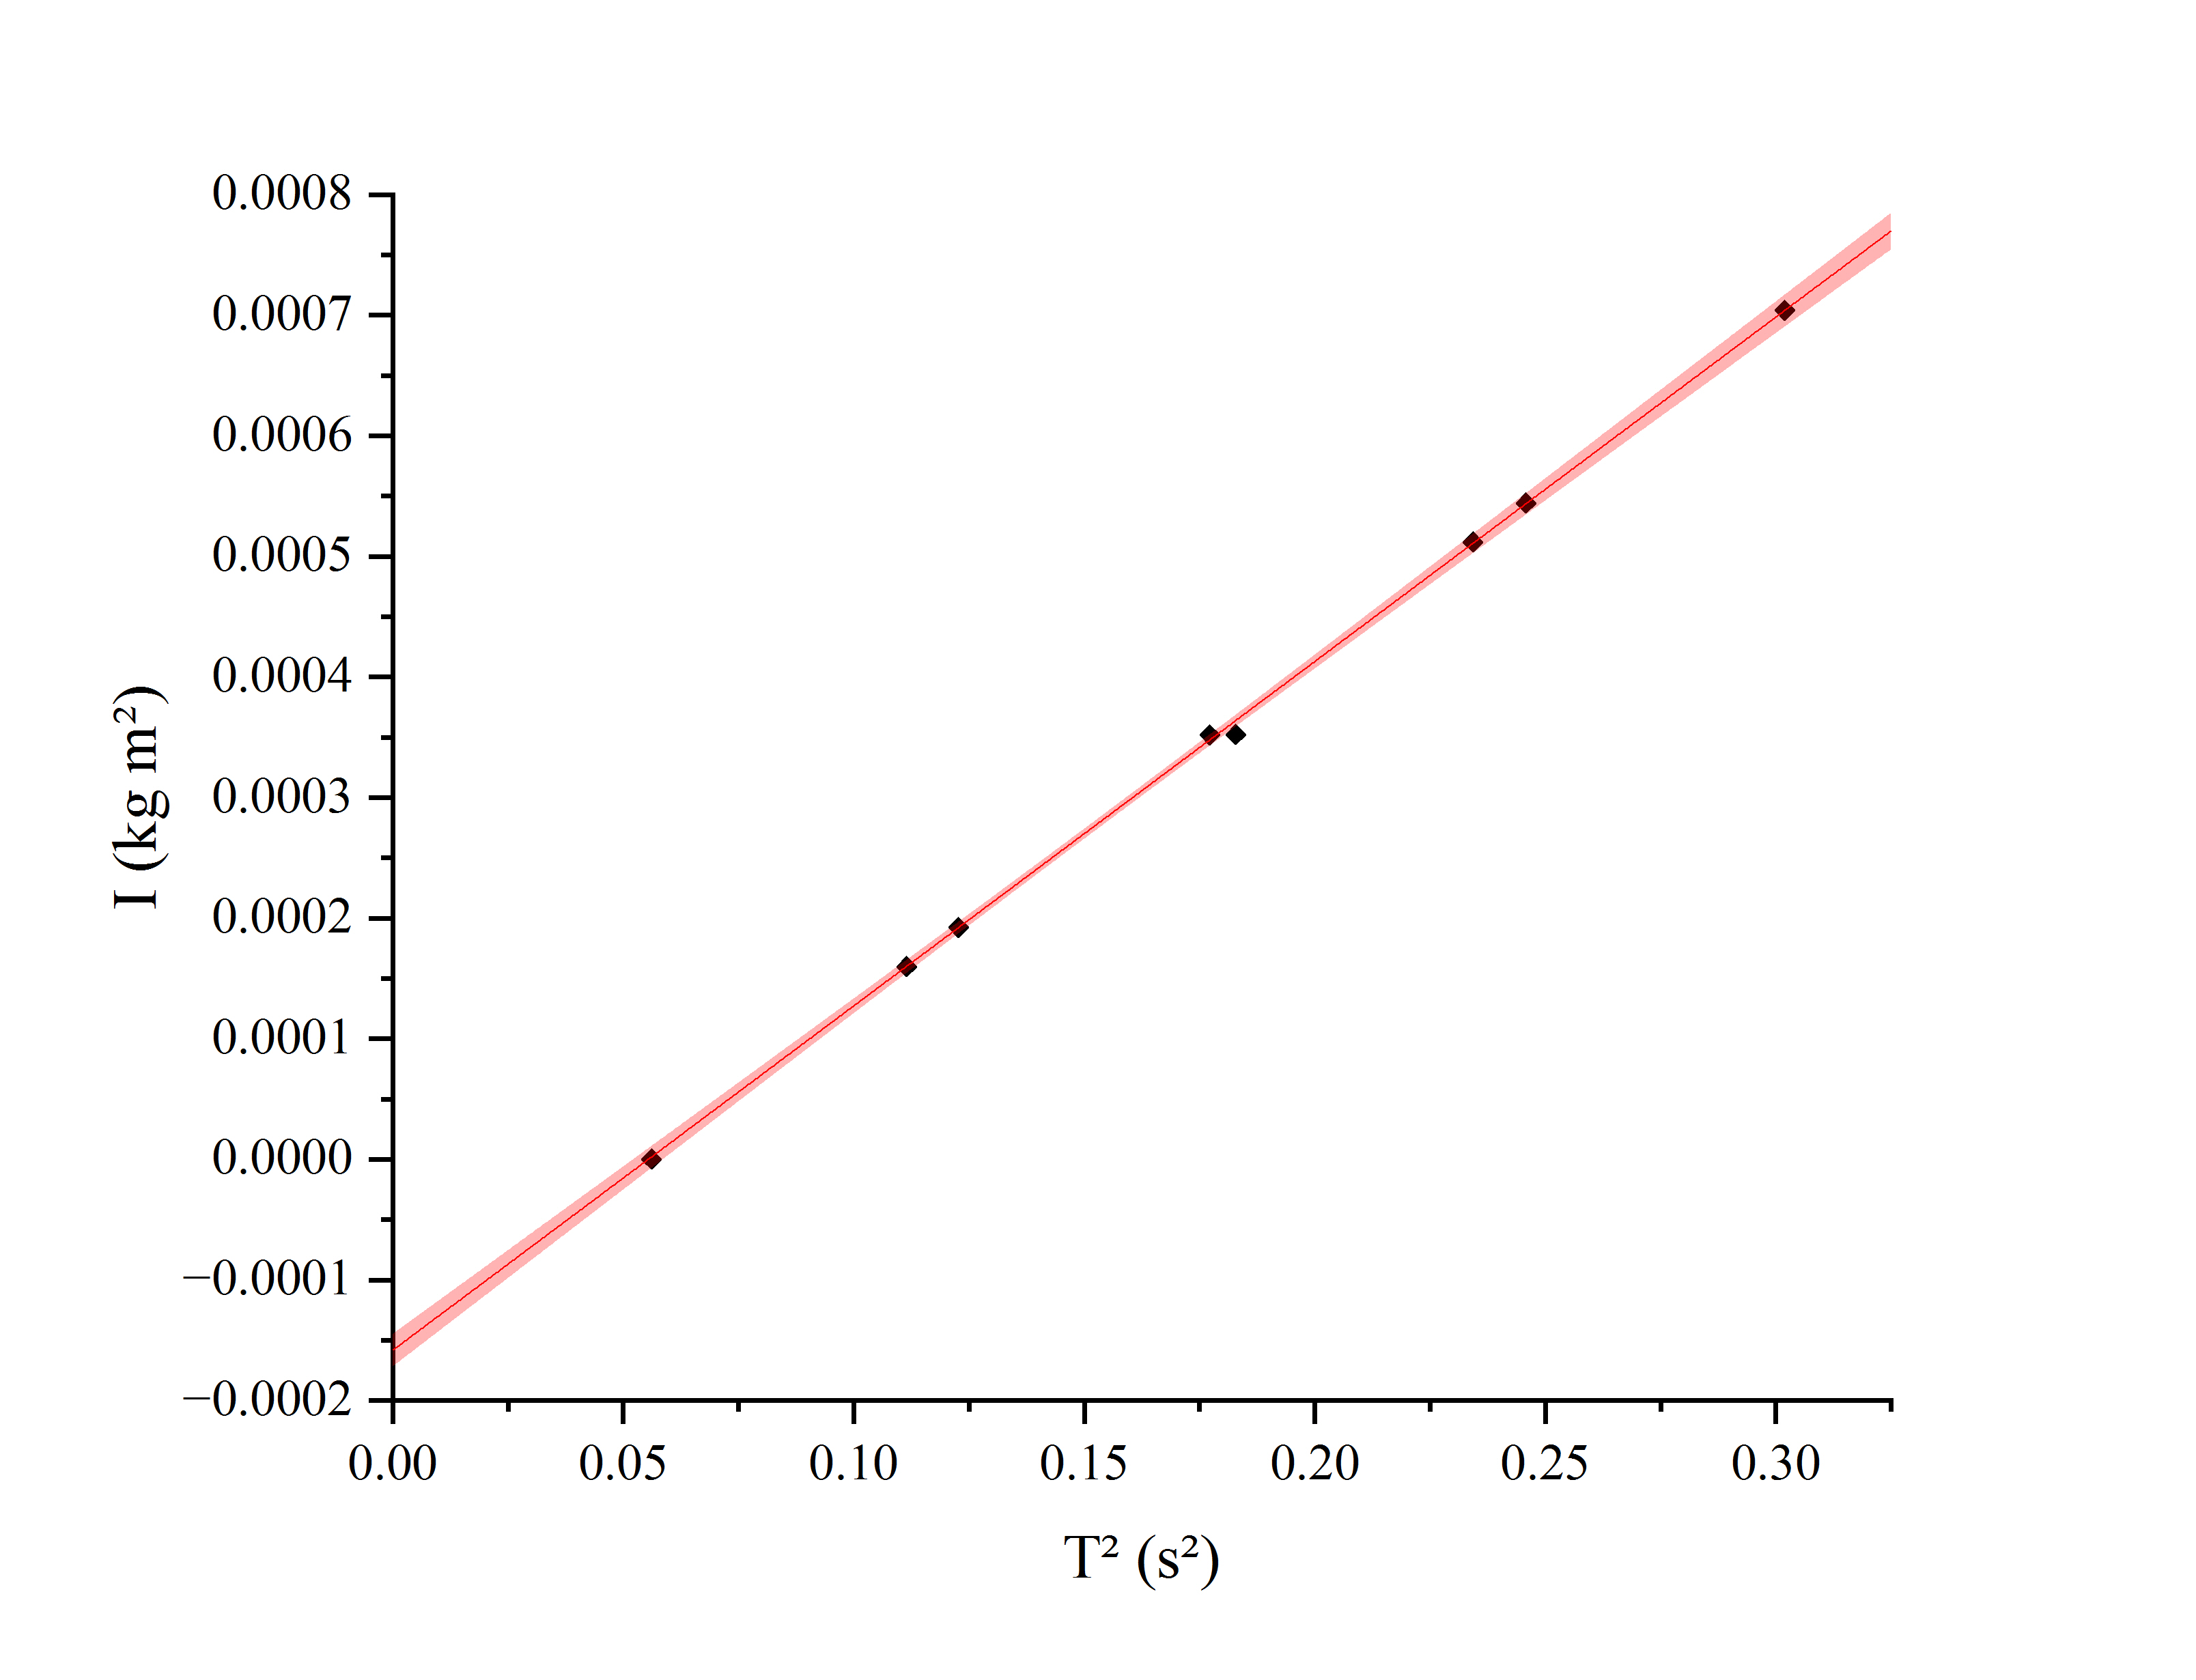
\includegraphics[trim={1.4cm .5cm 3.1cm 2.1cm},clip,width=.5\textwidth]{img/Reg3.jpg}
        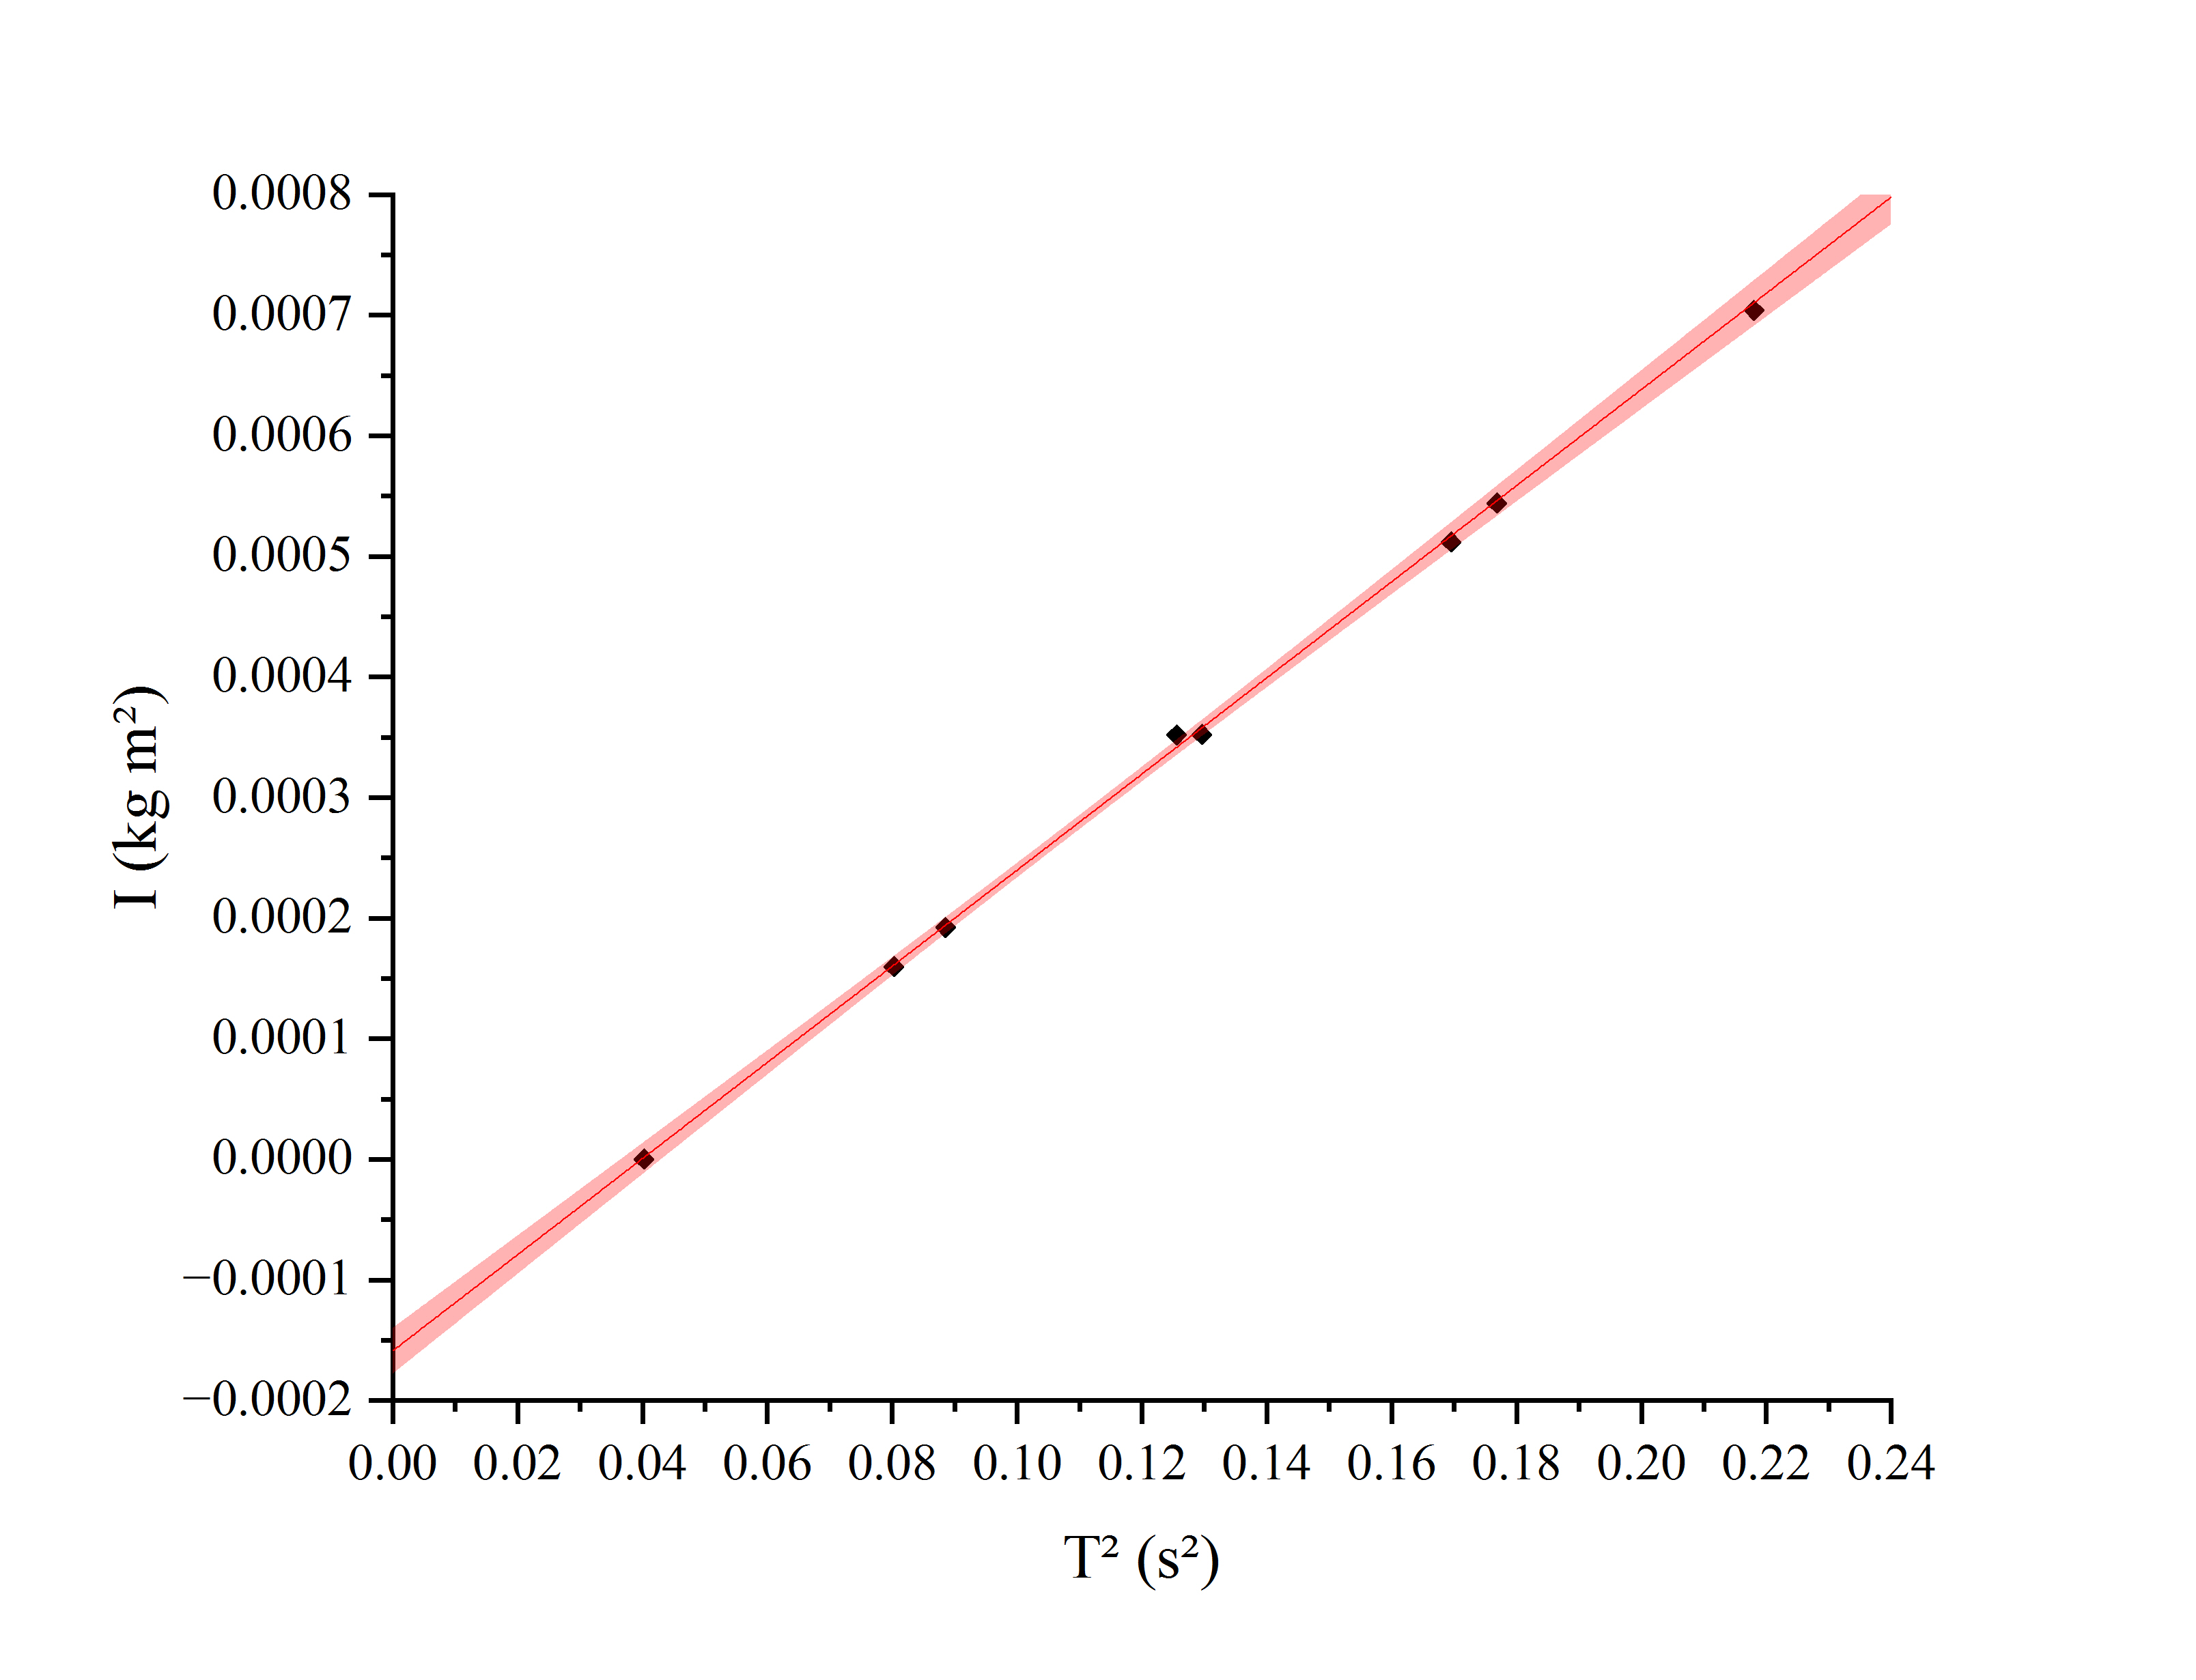
\includegraphics[trim={1.4cm .5cm 3.1cm 2.1cm},clip,width=.5\textwidth]{img/Reg4.jpg}
        \caption{\emph{
            I dati raccolti, assieme alle rette di regressione lineare
            (in rosa, le regioni di incertezza).
        }}
    \end{figure}
\end{center}

Riportiamo di seguito i risultati delle regressioni lineari,
dove $\xi=\frac{C}{4\pi^2}$ è il coefficiente angolare.

\begin{center}
\begin{tblr}{ |c|c|c|c| }
    \hline
    $j$ & $I_0$ ($10^{-4}\,\unit{kg\,m^2}$) & $\xi$ ($10^{-4}\,\unit{J}$) & $C$ ($\unit{mJ}$) \\
    \hline
    1 & $1.620\pm0.006$ & $2.015\pm0.002$ & $7.956\pm0.010$ \\
    2 & $1.581\pm0.006$ & $9.587\pm0.012$ & $37.85\pm0.05$  \\
    3 & $1.582\pm0.006$ & $28.56\pm0.03$  & $112.75\pm0.14$ \\
    4 & $1.587\pm0.006$ & $39.86\pm0.05$  & $157.38\pm0.20$ \\
    \hline
\end{tblr}
\end{center}

La costante torsionale $C$ dipende da caratteristiche del filo, come la lunghezza
$l$ e il diametro $d$. In particolare, vale:
\[
C = \frac{\pi}{2 l}\!\left(\frac{d}{2}\right)^{\!\!4}\!G = \frac{\pi d^4}{32 l} G
\]
dove la grandezza $G$ (dimensionalmente, una pressione) è detta
“modulo di scorrimento” del materiale di cui è composto il filo. Allora:
\[G = \frac{32 l}{\pi d^4} C\]
Di seguito riportiamo, in una tabella, le misure di $l$ e $d$ dei vari fili e i
corrispondenti valori della costante di scorrimento.

\begin{center}
\begin{tblr}{ |c|c|c|c|c| }
    \hline
    $j$ & $l$ ($\unit{cm}$) & $d$ ($\unit{mm}$) & $C$ ($\unit{mJ}$) & $G$ ($\unit{GPa}$) \\
    \hline
    1 & $43.3\pm0.1$ & $0.81\pm0.01$ & $7.956\pm0.010$ & $82\pm4$ \\
    2 & $43.1\pm0.1$ & $1.20\pm0.01$ & $37.85\pm0.05$  & $80\pm3$ \\
    3 & $43.0\pm0.1$ & $1.57\pm0.01$ & $112.75\pm0.14$ & $81\pm2$ \\
    4 & $42.7\pm0.1$ & $1.97\pm0.01$ & $157.38\pm0.20$ & $45.4\pm1.1$ \\
    \hline
\end{tblr}
\end{center}

Per valutare numericamente la consistenza dei risultati ottenuti con i valori
$G$ riportati in letteratura ($G_l$),
abbiamo calcolato, per ogni filo $j$, il seguente valore (numero puro):
\[\varepsilon = \frac{{G_j}_\text{best} - {G_l}_\text{best}}
                     {\delta G_j + \delta G_l}\]
Allora $G_j$ è consistente con $G_l$ se e solo se $\left|\varepsilon\right|\le 1$.

\begin{center}
\begin{tblr}{ |c|c|c|c|c| }
    \hline
    $j$ & $G_i$ ($\unit{GPa}$) & Materiale & $G_l$ ($\unit{GPa}$) & $\varepsilon$ \\
    \hline
    1 & $82\pm4$ &         &          & $-0.468$ \\
    2 & $80\pm3$ & Acciaio & $84\pm1$ & $-0.978$ \\
    3 & $81\pm2$ &         &          & $-0.809$ \\
    \hline[dashed]
    4 & $45.4\pm1.1$ & Rame& $43\pm1$ & $+1.174$ \\
    \hline
\end{tblr}
\end{center}

\subsection{Attrito}

Il moto del pendolo di torsione è condizionato dalla presenza
di attriti, che ne riducono l'ampiezza. In particolare, il modello
di riferimento è il seguente:
\[\theta(t) = \theta_0\cos(\omega t)\,e^{-\lambda t}\]
dove $\lambda$ è un parametro legato, appunto, agli attriti.
Per stimare $\lambda$, il gruppo di lavoro ha proceduto
su un'acquisizione come segue:
\begin{enumerate}
    \item
        Per prima cosa, abbiamo calcolato $\left|\theta(t)\right|$.
        Ciò ci ha permesso di trattare massimi e minimi “insieme”,
        evitando di ripetere l'analisi.
    \item
        Poi, abbiamo individuato i massimi dei nostri dati, ovvero
        gli insiemi di punti della forma
        $\left\{t_i,t_{i+1},\dots,t_j\right\}\times\left\{\left|\theta_k\right|\right\}$
        tali che $\left|\theta_{i-1}\right| < \left|\theta_k\right| > \left|\theta_{j+1}\right|$.
    \item
        Per ogni massimo, ne abbiamo calcolato il punto medio,
        prendendo come $\delta t_\text{picco}$ la semidispersione $\frac{1}{2}(t_j - t_i) + \delta t$.
    \item
        Infine, abbiamo graficato i punti su scala logaritmica e
        abbiamo effettuato una regressione lineare (pesata\footnote{
            $\delta\ln{\left|\theta\right|}$, infatti, varia molto,
            nonostante $\delta\left|\theta\right|$ sia costante.
            Ciò è conseguenza della propagazione degli errori.
        })
        sulle nuove ordinate.
\end{enumerate}


\begin{center}
    \begin{figure}[H]
        % trim={< v > ^}
        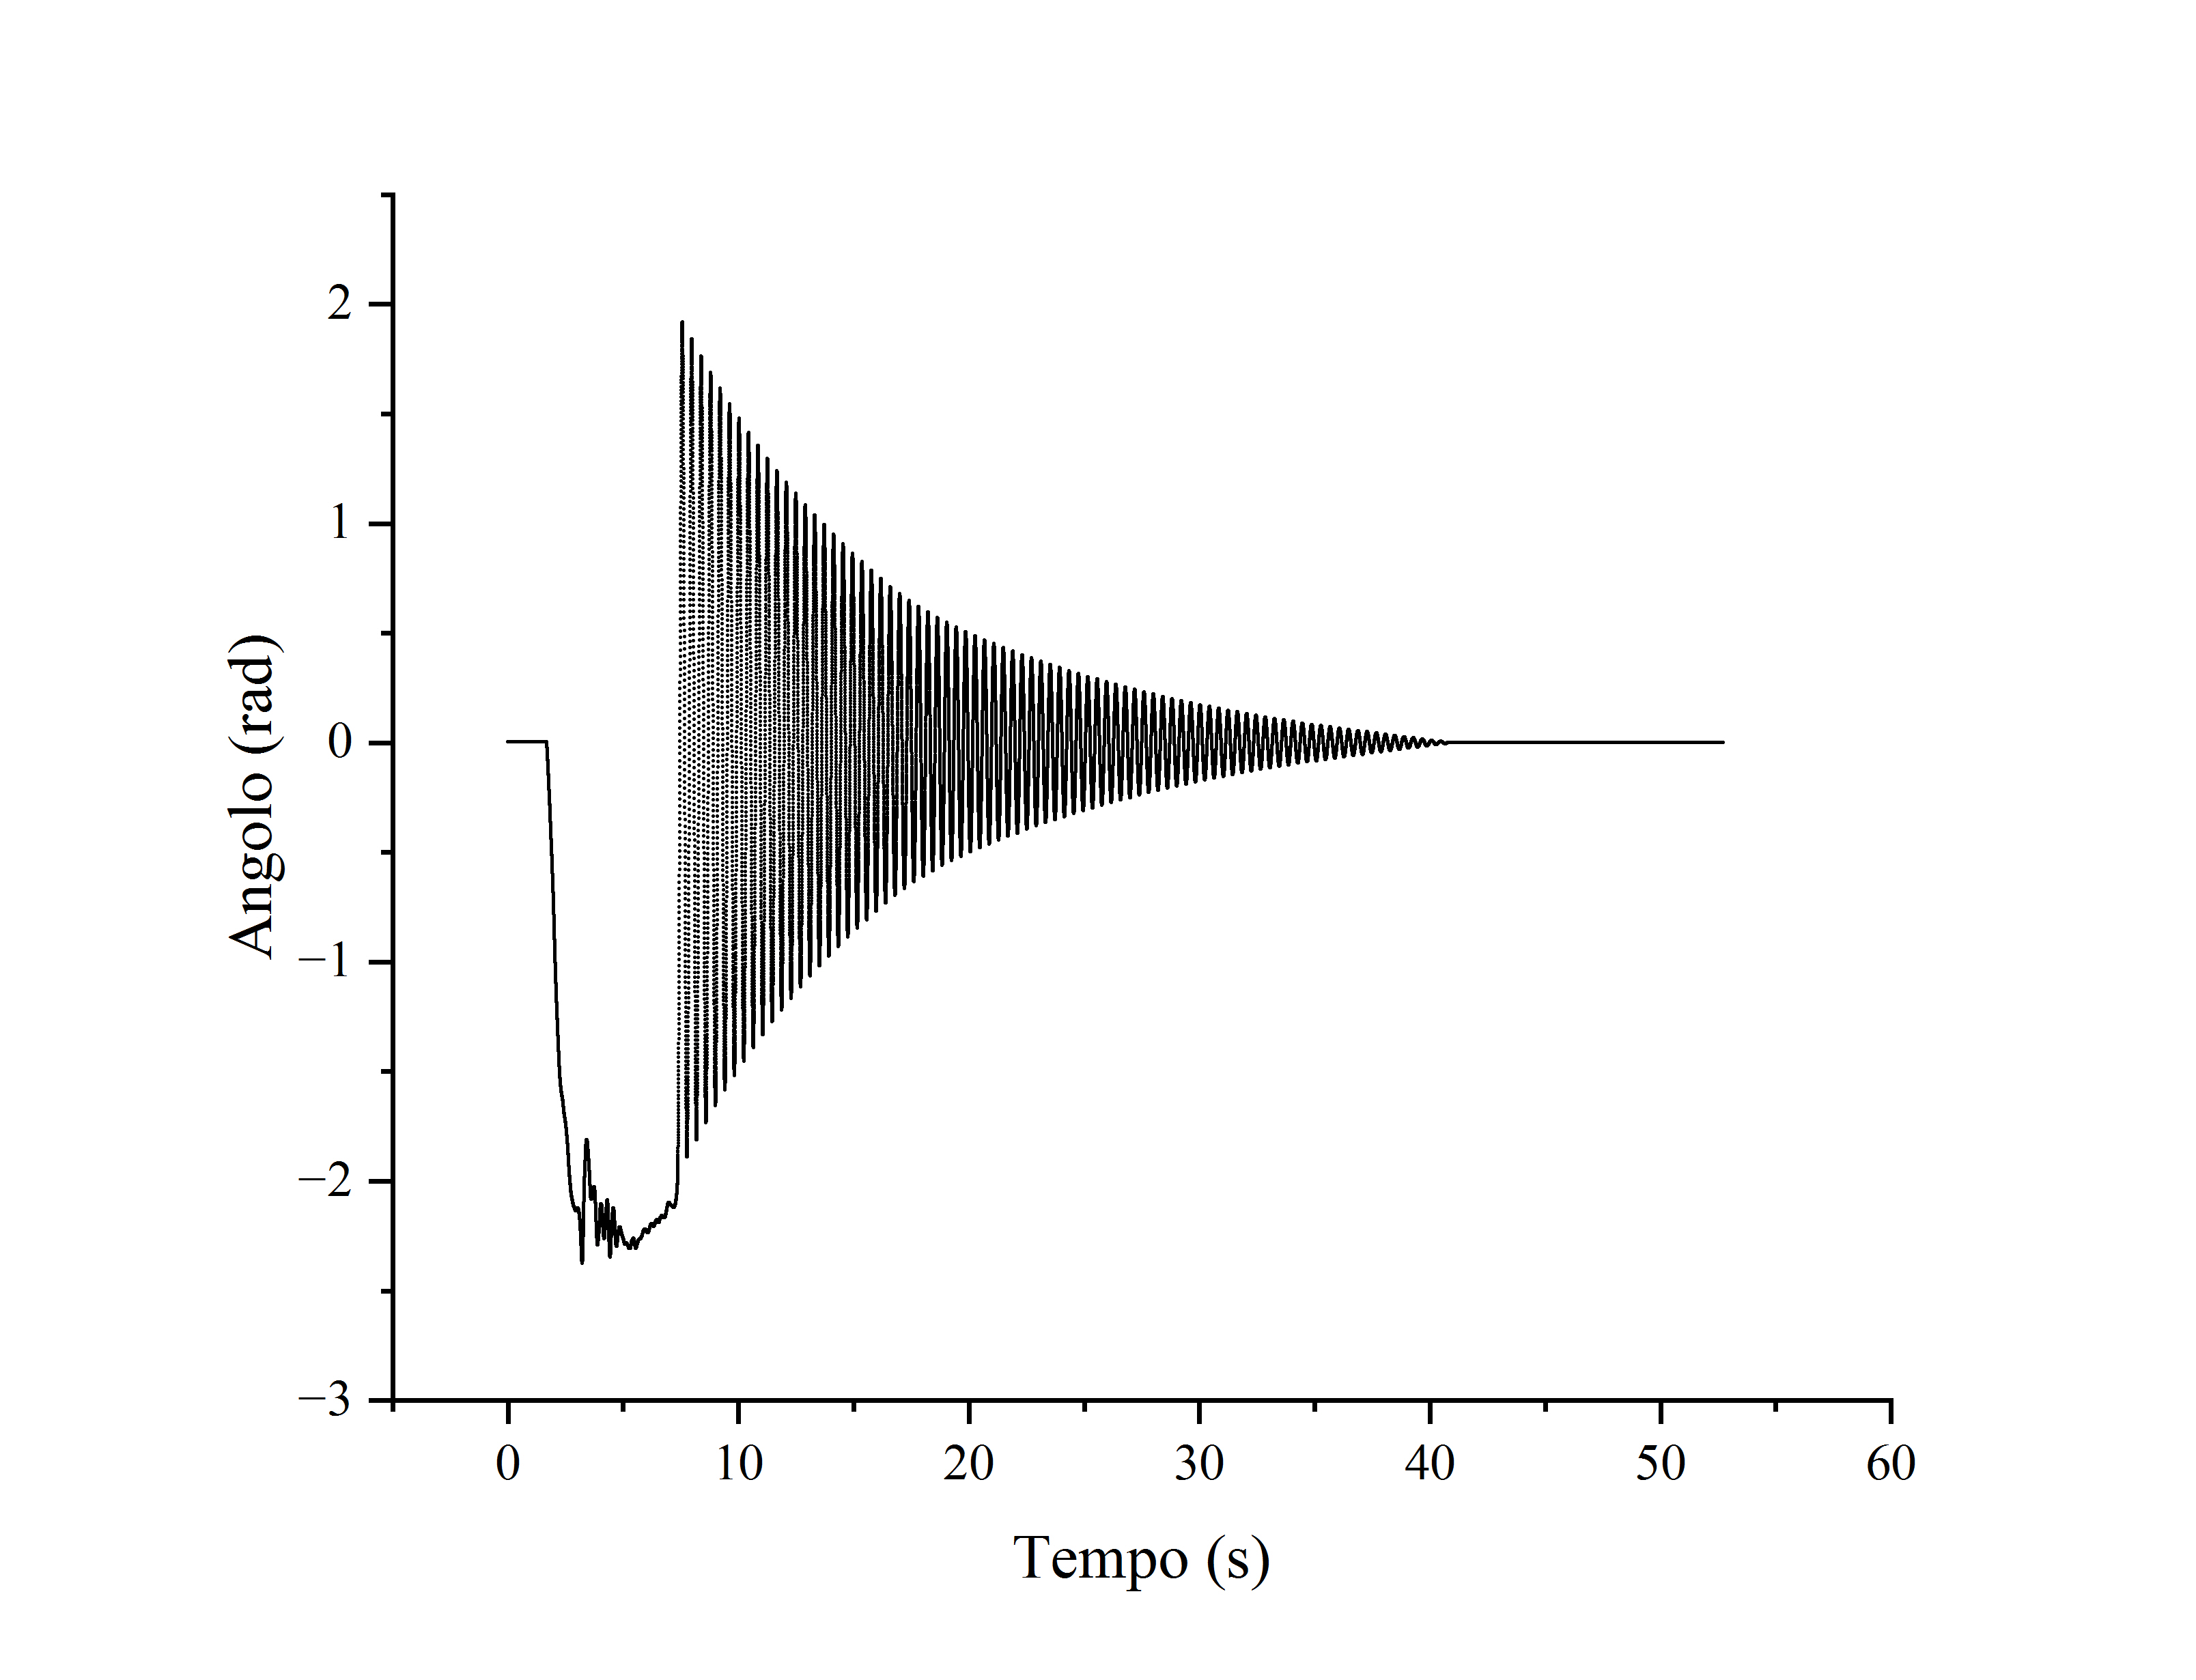
\includegraphics[trim={2cm 1cm 2cm 2.1cm},clip,width=\textwidth]{img/Exp1.jpg}
        \caption[]{\emph{I dati raccolti col termometro.
        In blu, la curva esponenziale così ottenuta.
        In verde, la temperatura ambiente.
        }}
    \end{figure}
\end{center}
\begin{center}
    \begin{figure}[H]
        % trim={< v > ^}
        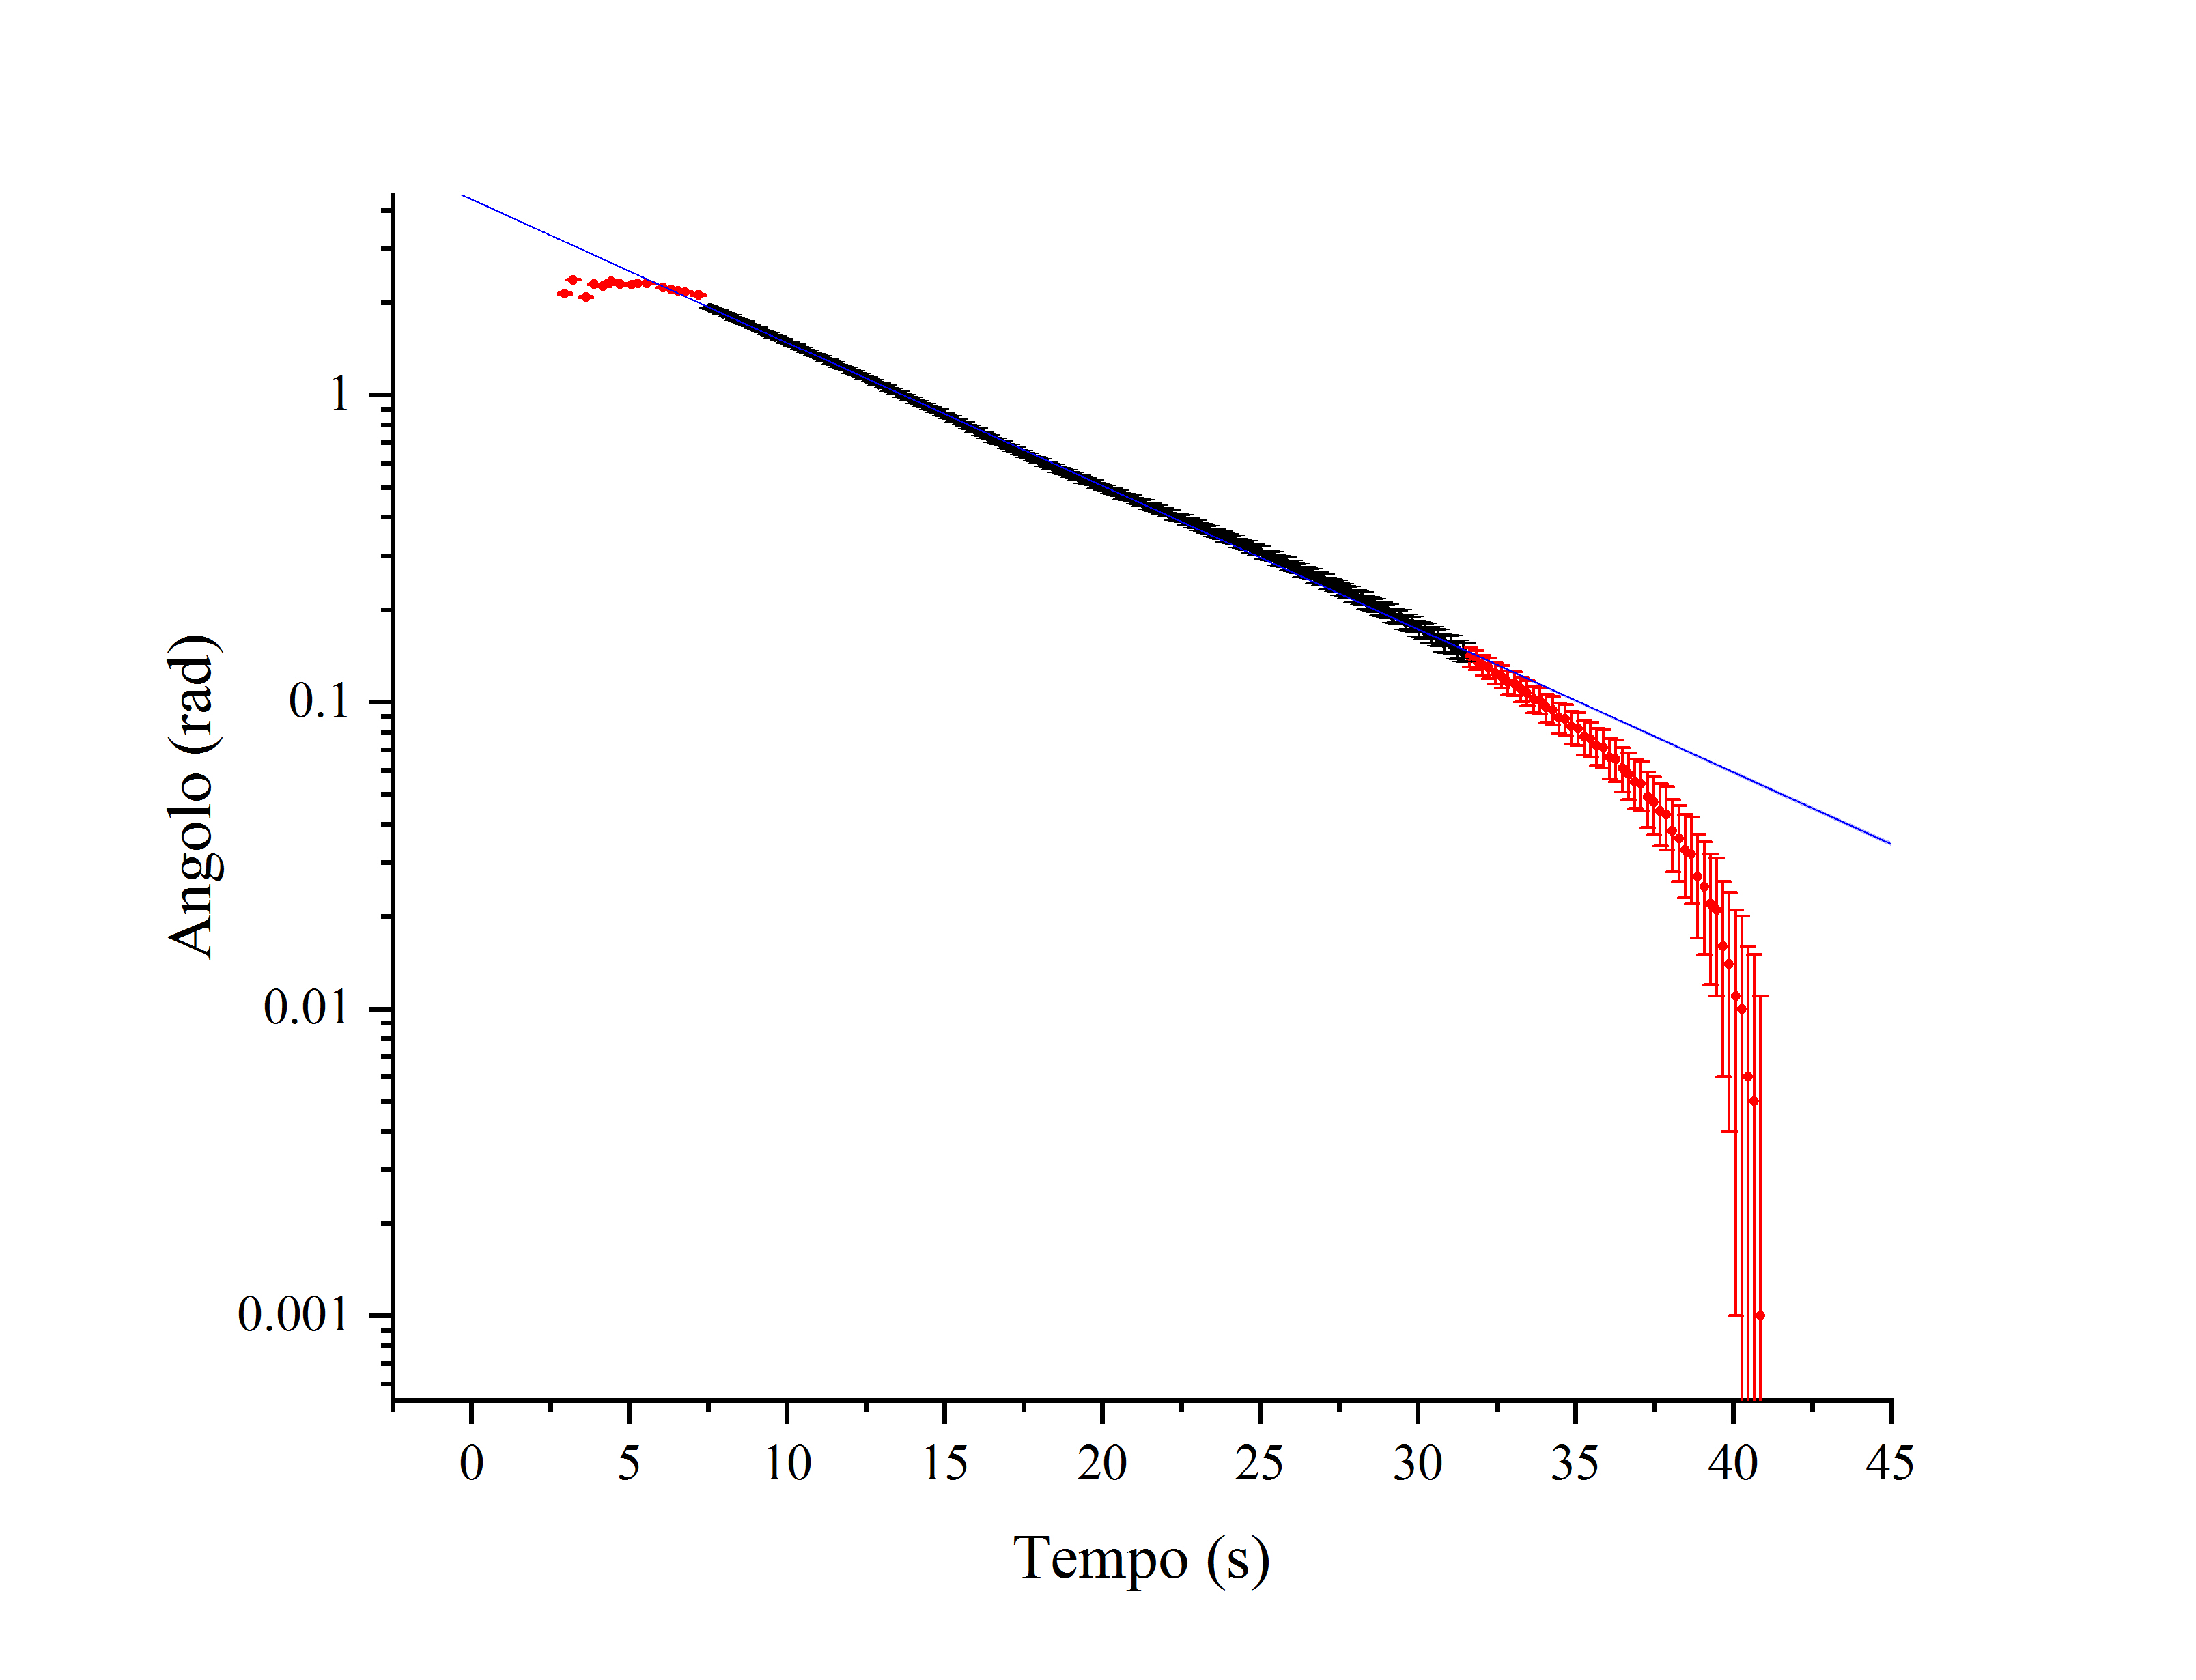
\includegraphics[trim={2cm 1cm 2cm 2.1cm},clip,width=\textwidth]{img/Exp4.jpg}
        \caption[]{\emph{I dati raccolti col termometro.
        In blu, la curva esponenziale così ottenuta.
        In verde, la temperatura ambiente.
        }}
    \end{figure}
\end{center}

\end{document}
